\documentclass[11pt]{beamer}

\usepackage{array}    % <-- For defining new column types
\usepackage{booktabs}
\usepackage{hyperref}
\usepackage{makecell} % <-- For multi-line cells
\usepackage[default]{opensans} 
\usepackage{pgffor}
\usepackage{pdfpages}
\usepackage{palatino}  
\usepackage{tcolorbox} 
\usepackage{textcomp}
\usepackage{ulem}
\usepackage{xcolor} 
\usepackage{tcolorbox} 
\usepackage{tikz}
\usepackage{tabularx}



\usetikzlibrary{arrows.meta} 
\usetikzlibrary{decorations.pathreplacing} 
\usetikzlibrary{decorations.pathmorphing}  
\usetikzlibrary{decorations.markings}     
\usetikzlibrary{decorations.text}      

\usepackage{listings}
\lstset{
  basicstyle=\ttfamily\small,
  columns=fullflexible,
  breaklines=true,
  frame=single,
  showstringspaces=false,
  showspaces=false,
  keepspaces=true,
  tabsize=4
}


\newtcbox{\highlighttexttt}{nobeforeafter, colframe=white, colback=lightgray!30, boxrule=0pt, arc=2pt, boxsep=0pt, left=1pt, right=1pt, top=1pt, bottom=1pt}
\newcommand{\hl}[1]{\colorbox{lightgray!30}{\texttt{#1}}}
\newcommand{\blink}[2]{\href{#1}{\textcolor{blue}{\underline{#2}}}}
\newcommand{\try}[1]{Have A Try: \blink{https://github.com/FSU-COP4610-F25/in-class-code}{#1}}

\usetheme{Madrid}
\usefonttheme{default} 

\useinnertheme{circles}

\setbeamertemplate{footline}{
    \leavevmode%
    \hbox{%
        \begin{beamercolorbox}[wd=0.92\paperwidth,ht=2.5ex,dp=1ex,left]{section in head/foot}
            \hspace{0.5em}
            \insertsectionnavigationhorizontal{0.9\paperwidth}{}{}
        \end{beamercolorbox}%
        \begin{beamercolorbox}[wd=0.08\paperwidth,ht=2.5ex,dp=1ex,right]{section in head/foot}
            \insertframenumber{} / \inserttotalframenumber
            \hspace{0.2em}
        \end{beamercolorbox}%
    }%
    \vskip0pt%
}


\setbeamersize{text margin left=1em, text margin right=1em}

\setbeamertemplate{frametitle}{
    \vspace{-0.5em} 
    \begin{beamercolorbox}[wd=\paperwidth,ht=2.5ex,dp=0.75ex,left]{frametitle} 
        \usebeamerfont{frametitle}\hspace{0.72em}\insertframetitle
    \end{beamercolorbox}
    \vspace{-0.5em} 
}


\newcommand{\FSUOSMeta}{%
  \author[Xin Liu]{\small Xin Liu}%
  \institute[FSU]{\small Florida State University\\[2pt]
    \href{mailto:xliu15@fsu.edu}{xliu15@fsu.edu}}%
  \date[\today]{\small CIS 4930/5930 Future Edge Networks\\[2pt]
    {\footnotesize\href{https://xinliulab.github.io/FSU-CIS4930-CIS5930-Future-Edge-Networks/}
         {\mbox{xinliulab.github.io/FSU-CIS4930-CIS5930-Future-Edge-Networks}}}}%
}

%!TEX root = ./main.tex

\usetikzlibrary{positioning,fit,backgrounds}

\definecolor{ranblue}{RGB}{46,91,186}
\definecolor{coreorange}{RGB}{222,122,36}
\definecolor{ranpurple}{RGB}{109,53,151}
\definecolor{softgreen}{RGB}{73,139,74}
\definecolor{softgray}{RGB}{92,98,105}

\newcommand{\source}[2]{%
  \par\vspace{0.25em}%
  {\tiny\textcolor{gray}{\href{#1}{\underline{#2}}}\par}%
}

% Inline expansion of an acronym at first use: SMS \expand{Short Message Service}
\newcommand{\expand}[1]{\textcolor{softgray}{(#1)}}

% Small gray glossary line, for slides with several acronyms at once.
\newcommand{\glossline}[1]{%
  \par\vspace{0.4em}%
  {\scriptsize\color{softgray}\raggedright#1\par}%
}

\newcommand{\plainterm}[2]{%
  \textbf{#1}\hspace{0.25em}{\small\textcolor{softgray}{#2}}%
}

\newcommand{\ask}[1]{%
  \begin{tcolorbox}[colback=blue!4,colframe=ranblue,boxrule=0.7pt,arc=2pt,
    left=5pt,right=5pt,top=4pt,bottom=4pt]
    \centering\large #1
  \end{tcolorbox}%
}

% Font is deliberately \normalsize, not \large: at \large a one-sentence takeaway
% wraps to two lines and the box grows into whatever is below it.
\newcommand{\takeaway}[1]{%
  \begin{tcolorbox}[colback=orange!7,colframe=coreorange,boxrule=0.7pt,arc=2pt,
    left=5pt,right=5pt,top=4pt,bottom=4pt]
    \centering\normalsize #1
  \end{tcolorbox}%
}

% Beamer overlays inside TikZ: \visible<...> breaks path parsing inside node text,
% so reveal nodes with the standard opacity idiom instead: \node[visible on=<2->] ...
\tikzset{
  invisible/.style={opacity=0,text opacity=0},
  visible on/.style={alt=#1{}{invisible}},
  alt/.code args={<#1>#2#3}{\alt<#1>{\pgfkeysalso{#2}}{\pgfkeysalso{#3}}},
}

\tikzset{
  netnode/.style={draw=ranblue,fill=blue!5,rounded corners=3pt,
    minimum width=1.9cm,minimum height=0.82cm,align=center,font=\bfseries},
  corenode/.style={draw=coreorange,fill=orange!7,rounded corners=3pt,
    minimum width=1.9cm,minimum height=0.82cm,align=center,font=\bfseries},
  oranode/.style={draw=ranpurple,fill=purple!6,rounded corners=3pt,
    minimum width=1.9cm,minimum height=0.82cm,align=center,font=\bfseries},
  flow/.style={-{Latex[length=2.4mm]},thick,draw=softgray}
}

% Full-width question/answer block: spans the whole frame, no box.
% Use below \end{columns} when the question is meant for the whole slide.
\newcommand{\qa}[2]{%
  \par\vspace{0.55em}%
  {\large\raggedright
    \noindent\hangindent=1.25em\hangafter=1
    \textcolor{ranblue}{\textbf{Q:}}\hspace{0.35em}\textbf{#1}\par
    \vspace{0.35em}
    \noindent\hangindent=1.25em\hangafter=1
    \textcolor{coreorange}{\textbf{A:}}\hspace{0.35em}#2\par}%
}

% Repeating template for "this box is gone in the next diagram" frames.
% The deck's spine: a term never vanishes between two architecture diagrams
% without a frame explaining the pressure that removed it.
% #1 what it did, #2 what broke, #3 what replaced it
\newcommand{\gonebox}[3]{%
  \vspace{0.5em}%
  \begin{columns}[T,onlytextwidth]
    \column{0.30\textwidth}
      {\small\textbf{\textcolor{softgray}{What it did}}\par}
      \vspace{0.4em}
      {\small #1\par}
    \column{0.34\textwidth}
      {\small\textbf{\textcolor{coreorange}{What broke}}\par}
      \vspace{0.4em}
      {\small #2\par}
    \column{0.30\textwidth}
      {\small\textbf{\textcolor{softgreen}{What replaced it}}\par}
      \vspace{0.4em}
      {\small #3\par}
  \end{columns}%
}

%!TEX root = ./main.tex

% Styles added for this deck; ran_macros.tex stays identical to the Wi-Fi History copy.

% Navigation symbols sit on top of the source lines at the bottom right.
\setbeamertemplate{navigation symbols}{}

\tikzset{
  % The physical channel: gray, so it reads as "not designed by us".
  chnode/.style={draw=softgray,fill=gray!10,rounded corners=3pt,
    minimum width=1.7cm,minimum height=0.82cm,align=center,font=\bfseries},
  % Shared knowledge / trained model: green, used only for what both ends must hold.
  kbnode/.style={draw=softgreen,fill=green!7,rounded corners=3pt,
    minimum width=1.9cm,minimum height=0.82cm,align=center,font=\bfseries},
  % Learned (neural) blocks: purple, so "trained" is visible at a glance.
  nnnode/.style={draw=ranpurple,fill=purple!6,rounded corners=3pt,
    minimum width=1.9cm,minimum height=0.82cm,align=center,font=\bfseries},
  % Plain content boxes (photo, sentence, answer).
  endnode/.style={draw=softgray,fill=gray!6,rounded corners=3pt,
    minimum width=1.7cm,minimum height=1.0cm,align=center,font=\small\bfseries},
  lbl/.style={font=\scriptsize,text=softgray,align=center},
  iface/.style={font=\scriptsize\bfseries,text=coreorange},
}

% A tiny street-scene video frame (sky, road, one pedestrian, one car), drawn at
% (0,0)--(3.4,2.1). Used on the "lost block" slide.
\tikzset{
  streetframe/.pic={
    \fill[blue!12] (0,1.0) rectangle (3.4,2.1);
    \fill[gray!25] (0,0) rectangle (3.4,1.0);
    \draw[white,thick,dashed] (0,0.45) -- (3.4,0.45);
    \fill[coreorange] (1.15,1.36) circle (0.13);
    \fill[coreorange] (1.03,0.72) rectangle (1.27,1.21);
    \fill[ranblue!70,rounded corners=1pt] (2.25,0.18) rectangle (3.1,0.58);
    \draw[softgray] (0,0) rectangle (3.4,2.1);
  }
}

% Step-by-step reveal for the colored boxes. A tcolorbox inside \uncover would still
% paint its background, so on earlier overlays draw a fully transparent copy instead:
% the box keeps its space and nothing below it jumps when it appears.
% Usage: \takeawayat{3-}{text}   \askat{2-}{text}
\newcommand{\takeawayghost}[1]{%
  \begin{tcolorbox}[colback=orange!7,colframe=coreorange,boxrule=0.7pt,arc=2pt,
    left=5pt,right=5pt,top=4pt,bottom=4pt,
    opacityback=0,opacityframe=0,opacitytext=0]
    \centering\normalsize #1
  \end{tcolorbox}%
}
\newcommand{\askghost}[1]{%
  \begin{tcolorbox}[colback=blue!4,colframe=ranblue,boxrule=0.7pt,arc=2pt,
    left=5pt,right=5pt,top=4pt,bottom=4pt,
    opacityback=0,opacityframe=0,opacitytext=0]
    \centering\large #1
  \end{tcolorbox}%
}
\newcommand{\takeawayat}[2]{\alt<#1>{\takeaway{#2}}{\takeawayghost{#2}}}
\newcommand{\askat}[2]{\alt<#1>{\ask{#2}}{\askghost{#2}}}

% Citation line in the same style as \source, for references with no stable open URL.
\newcommand{\plainsource}[1]{%
  \par\vspace{0.25em}%
  {\tiny\textcolor{gray}{#1}\par}%
}

% Picture-based "signal gets weaker" sketches (slides "Where it struggles" and
% "Weak signal: blurrier, not frozen"). All frames use the streetframe geometry.
% \signalbars{x}{y}{n}: four bars at (x,y), the first n filled.
\newcommand{\signalbars}[3]{%
  \foreach \i in {1,2,3,4}{%
    \ifnum\i>#3\relax
      \draw[softgray,thick] (#1+0.22*\i,#2) rectangle ++(0.14,0.12*\i);
    \else
      \fill[ranblue] (#1+0.22*\i,#2) rectangle ++(0.14,0.12*\i);
    \fi}%
}
% Pedestrian and car at a given opacity, so blurred frames can stack shifted copies.
\newcommand{\streetobjects}[1]{%
  \fill[coreorange,opacity=#1] (1.15,1.36) circle (0.13);
  \fill[coreorange,opacity=#1] (1.03,0.72) rectangle (1.27,1.21);
  \fill[ranblue!70,opacity=#1,rounded corners=1pt] (2.25,0.18) rectangle (3.1,0.58);%
}
\tikzset{
  % today's link below its threshold: the picture stops
  frozen/.pic={
    \fill[black,opacity=0.6] (0,0) rectangle (3.4,2.1);
    \fill[white] (1.45,0.85) rectangle (1.6,1.45);
    \fill[white] (1.8,0.85) rectangle (1.95,1.45);
    \node[font=\small\bfseries,text=white] at (1.7,0.45) {frozen};
  },
  % today's link after feedback lowered the bitrate: coarser, blockier picture
  streetblocky/.pic={
    \fill[blue!12] (0,1.0) rectangle (3.4,2.1);
    \fill[gray!25] (0,0) rectangle (3.4,1.0);
    \fill[coreorange!85] (0.98,1.2) rectangle (1.32,1.54);
    \fill[coreorange!85] (0.98,0.68) rectangle (1.32,1.2);
    \fill[ranblue!60] (2.2,0.12) rectangle (3.15,0.64);
    \draw[white,opacity=0.55] (0,0) grid[step=0.34] (3.4,2.1);
    \draw[softgray] (0,0) rectangle (3.4,2.1);
  },
  % today's link right after a sudden drop, before feedback reacts: frames arrive late
  late/.pic={
    \fill[black,opacity=0.45] (0,0) rectangle (3.4,2.1);
    \draw[white,very thick] (1.7,1.25) circle (0.38);
    \draw[white,very thick] (1.7,1.25) -- (1.7,1.5);
    \draw[white,very thick] (1.7,1.25) -- (1.88,1.25);
    \node[font=\small\bfseries,text=white] at (1.7,0.45) {late};
  },
  % Version 3: coarse background, sharp pedestrian (bits spent where the task looks)
  streetv3/.pic={
    \fill[blue!12] (0,1.0) rectangle (3.4,2.1);
    \fill[gray!25] (0,0) rectangle (3.4,1.0);
    \fill[ranblue!60] (2.2,0.12) rectangle (3.15,0.64);
    \draw[white,opacity=0.55] (0,0) grid[step=0.34] (3.4,2.1);
    \fill[blue!12] (0.82,1.0) rectangle (1.48,1.68);
    \fill[gray!25] (0.82,0.58) rectangle (1.48,1.0);
    \fill[coreorange] (1.15,1.36) circle (0.13);
    \fill[coreorange] (1.03,0.72) rectangle (1.27,1.21);
    \draw[softgreen,thick] (0.82,0.58) rectangle (1.48,1.68);
    \draw[softgray] (0,0) rectangle (3.4,2.1);
  },
  % learned link with a weaker signal: same scene, softer
  streetsoft/.pic={
    \fill[blue!12] (0,1.0) rectangle (3.4,2.1);
    \fill[gray!25] (0,0) rectangle (3.4,1.0);
    \draw[white,thick,dashed,opacity=0.6] (0,0.45) -- (3.4,0.45);
    \foreach \dx/\dy in {-0.05/0,0.05/0,0/0.05,0/-0.05}{
      \begin{scope}[shift={(\dx,\dy)}]\streetobjects{0.35}\end{scope}}
    \draw[softgray] (0,0) rectangle (3.4,2.1);
  },
  streetblurry/.pic={
    \fill[blue!12] (0,1.0) rectangle (3.4,2.1);
    \fill[gray!25] (0,0) rectangle (3.4,1.0);
    \draw[white,thick,dashed,opacity=0.35] (0,0.45) -- (3.4,0.45);
    \foreach \dx/\dy in {-0.12/0,0.12/0,0/0.12,0/-0.12,-0.08/-0.08,0.08/0.08,
        -0.08/0.08,0.08/-0.08}{
      \begin{scope}[shift={(\dx,\dy)}]\streetobjects{0.2}\end{scope}}
    \draw[softgray] (0,0) rectangle (3.4,2.1);
  },
}


\title[Semantic Communication]{Class 17: Semantic Communication}
\subtitle{From Delivering Bits to Delivering Meaning and Tasks}

\FSUOSMeta

\begin{document}

\begin{frame}[plain]
  \titlepage
\end{frame}

\addtocounter{framenumber}{-1}

% TALK BUDGET: 50:00 = 3000 s over 23 content frames. Running example: one street
% camera's live video, watched by a person (A) and analyzed by an edge AI (B).
%   01 Intro                          0:00--2:20   1 frame   140 s
%   02 Today (bit pipe)               2:20--14:10  5 frames  710 s
%   03 What is SemCom + gains         14:10--22:10  4 frames  480 s
%   04 Version 1: reconstruction      22:10--30:30  4 frames  500 s
%   05 Version 2: task-oriented       30:30--39:40  4 frames  550 s
%   06 Version 3: meaning-aware bits  39:40--43:10  2 frames  210 s
%   07 Wrap-up                        43:10--50:00  3 frames  410 s
% Style: one idea per frame, few words; anything longer is revealed step by step.
% Technical detail and sources live in each frame's "Teaching note" comment.
%!TEX root = ./main.tex

\section[Intro]{Introduction}

% SECTION TIMING: 0:00--2:20 (1 frame).

% Teaching note (140 s): open with the picture and the question; do not answer it
% yet. Take one or two guesses. Receiver A needs the video itself; receiver B only
% needs to know where the pedestrians are. The whole lecture lives in the gap between
% those two receivers. Then reveal the route one line at a time.
\begin{frame}{One video stream, two receivers}
  \vspace{0.6em}
  \centering
  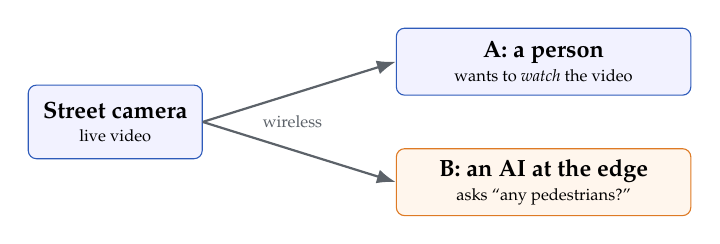
\begin{tikzpicture}[scale=0.85,transform shape]
    \node[netnode,minimum width=2.6cm,minimum height=1.1cm] (cam) at (0,0)
      {Street camera\\[-2pt]{\scriptsize\mdseries live video}};
    \node[netnode,minimum width=4.4cm,minimum height=1.0cm] (a) at (6.4,0.9)
      {A: a person\\[-2pt]{\scriptsize\mdseries wants to \textit{watch} the video}};
    \node[corenode,minimum width=4.4cm,minimum height=1.0cm] (b) at (6.4,-0.9)
      {B: an AI at the edge\\[-2pt]{\scriptsize\mdseries asks ``any pedestrians?''}};
    \draw[flow] (cam.east) -- (a.west);
    \draw[flow] (cam.east) -- (b.west);
    \node[lbl] at (2.65,0) {wireless};
  \end{tikzpicture}

  \vspace{0.5em}
  \askat{2-}{Do A and B need the same data?}

  \vspace{0.6em}
  \raggedright
  \begin{enumerate}[<+(2)->]\itemsep4pt
    \item Today: copy every bit of every frame
    \item Semantic communication: send the \textbf{meaning}
    \item Version 1: \textbf{rebuild} the video
    \item Version 2: just get the \textbf{task} done --- no video rebuilt
    \item Version 3: keep today's pipe, spend bits by \textbf{meaning}
  \end{enumerate}
\end{frame}

%!TEX root = ./main.tex

\section[Today]{How Communication Works Today}

% SECTION TIMING: 2:20--14:10 (5 frames): 130 + 190 + 130 + 90 + 170 = 710 s.
% Flex frame if running late: "Why this design won" compresses to 60 s (say the two
% ideas, skip the formula).

% Teaching note (130 s): redraw Shannon's Fig. 1 and name the five boxes (in the
% original figure the channel is an unlabeled box; the text names the five parts:
% source, transmitter, channel, receiver, destination). Shannon's problem: reproduce,
% at the destination, the message chosen at the source -- exactly or approximately.
% Then read the quote slowly; it is the hinge of the whole lecture. Shannon did not
% say meaning is unimportant, only that it is not needed to design the pipe.
% Information = which message was chosen out of all possible ones, counted in bits.
\begin{frame}{Shannon 1948: copy the message}
  \vspace{1.2em}
  \centering
  % SOURCE: Shannon, Bell Syst. Tech. J. 27 (1948), Fig. 1 and Introduction.
  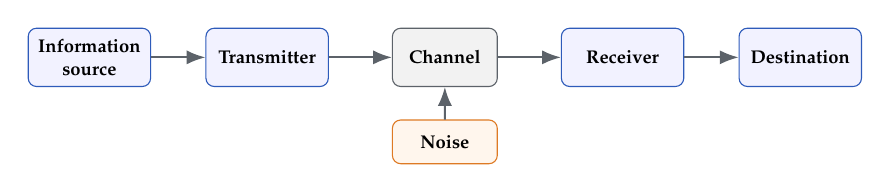
\begin{tikzpicture}[scale=0.74,transform shape,
      blk/.style={netnode,minimum width=2.1cm,minimum height=1.0cm,font=\small\bfseries}]
    \node[blk] (src) at (0,0) {Information\\source};
    \node[blk] (tx)  at (3.05,0) {Transmitter};
    \node[chnode,minimum width=1.8cm,minimum height=1.0cm,font=\small\bfseries] (ch)
      at (6.1,0) {Channel};
    \node[blk] (rx)  at (9.15,0) {Receiver};
    \node[blk] (dst) at (12.2,0) {Destination};
    \node[corenode,minimum width=1.8cm,minimum height=0.75cm,font=\small\bfseries]
      (noise) at (6.1,-1.45) {Noise};
    \draw[flow] (src) -- (tx);
    \draw[flow] (tx) -- (ch);
    \draw[flow] (ch) -- (rx);
    \draw[flow] (rx) -- (dst);
    \draw[flow] (noise) -- (ch);
  \end{tikzpicture}

  \vspace{1.0em}
  \uncover<2->{{\large Goal: an \textbf{exact copy} at the other end.}\par}

  \vspace{1.0em}
  \uncover<3->{{\itshape ``These semantic aspects of communication are irrelevant
    to the engineering problem.''}\par
    \vspace{0.2em}
    {\small\textcolor{softgray}{--- Shannon (1948)}}\par}

  \vspace{0.9em}
  \takeawayat{4-}{Meaning was left out on purpose:\\
    a bit is a bit, whatever it encodes.}
  \source{https://doi.org/10.1002/j.1538-7305.1948.tb01338.x}{C.\ E.\ Shannon,
    ``A Mathematical Theory of Communication,'' Bell Syst.\ Tech.\ J., 1948}
\end{frame}

% Teaching note (190 s): the suitcase analogy carries the slide. Compress = vacuum-pack
% the clothes (source coding; for video, a codec such as H.264 removes what is
% predictable inside each frame and between consecutive frames, so every bit left
% matters). Protect = bubble wrap (channel coding: add structured redundancy so the
% receiver can fix errors; modern examples are LDPC and polar codes -- the Wi-Fi
% lecture did not cover them, so just say "error-correcting code"). Send = the truck
% (modulation: the QAM and OFDM of the Wi-Fi lecture). The truck never opens the
% suitcase: each block is designed and upgraded on its own, and the halves agree on
% one interface only -- bits. The receiver undoes each step in reverse order.
% Fourth click plants FEEDBACK, which "Where it struggles" builds on: the receiver
% keeps reporting how the delivery is going, and the sender adjusts -- phone-call
% analogy: "you're breaking up", so you slow down and repeat. In real-time video
% (WebRTC) the receiver reports packet arrival times (TWCC) and the sender's
% congestion control (GCC) sets the encoder's target bitrate -- hence the arrow back
% to Compress. Wi-Fi itself also adapts at the Send step (it switches to slower,
% sturdier transmission settings); no need to say this unless asked.
\begin{frame}{Today's pipeline: like shipping a suitcase}
  \vspace{1.6em}
  \centering
  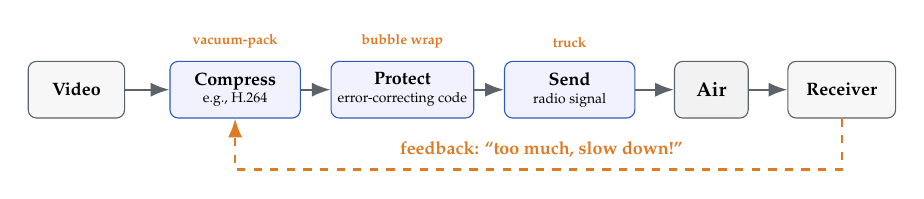
\begin{tikzpicture}[scale=0.72,transform shape,
      blk/.style={netnode,minimum width=2.3cm,minimum height=1.0cm,font=\small\bfseries}]
    \node[endnode] (src) at (0,0) {Video};
    \node[blk] (c) at (2.8,0) {Compress\\[-2pt]{\scriptsize\mdseries e.g., H.264}};
    \node[blk] (p) at (5.75,0) {Protect\\[-2pt]{\scriptsize\mdseries error-correcting code}};
    \node[blk] (s) at (8.7,0) {Send\\[-2pt]{\scriptsize\mdseries radio signal}};
    \node[chnode,minimum width=1.3cm,minimum height=1.0cm] (air) at (11.2,0) {Air};
    \node[endnode,minimum width=1.9cm] (rx) at (13.5,0) {Receiver};
    \draw[flow] (src) -- (c);
    \draw[flow] (c) -- (p);
    \draw[flow] (p) -- (s);
    \draw[flow] (s) -- (air);
    \draw[flow] (air) -- (rx);
    \node[iface,above=3pt of c,visible on=<2->] {vacuum-pack};
    \node[iface,above=3pt of p,visible on=<2->] {bubble wrap};
    \node[iface,above=3pt of s,visible on=<2->] {truck};
    \draw[flow,coreorange,dashed,visible on=<4->] (rx.south) -- ++(0,-0.9) -| (c.south);
    \node[font=\small\bfseries,text=coreorange,visible on=<4->] at (8.2,-1.05)
      {feedback: ``too much, slow down!''};
  \end{tikzpicture}

  \vspace{1.0em}
  \uncover<3->{{\large The truck never opens the suitcase.}\par}

  \vspace{0.5em}
  \uncover<4->{{\small\textcolor{softgray}{The receiver reports back, and the sender
    adjusts the video quality --- like ``you're breaking up'' on a phone call.}}\par}

  \vspace{1.0em}
  \takeawayat{5-}{Every block has one job:\\
    \textbf{deliver these bits exactly.}}
\end{frame}

% Teaching note (130 s): reveal one box at a time and do the arithmetic out loud.
% Raw: 1920 x 1080 pixels x 24 bits x 30 frames/s = 1.49 Gb/s. H.264 at 8 Mb/s: that
% is YouTube's recommended upload bitrate for 1080p SDR at 24/25/30 frames/s (YouTube
% Help, "YouTube recommended upload encoding settings"; 12 Mb/s at 48/50/60 frames/s)
% -- a realistic compressed rate, about 190x smaller than raw. Protection: the 802.11a
% 54 Mb/s mode uses a rate-3/4 convolutional code, i.e., +1/3 extra bits -> about
% 10.7 Mb/s on air, roughly 20% of an old 54 Mb/s Wi-Fi link, nonstop. The orange box
% is a TEACHING EXAMPLE: if B only needs a pedestrian count, 1 byte per frame x 30
% frames/s = 240 b/s. Q&A mechanism (unicast Wi-Fi frames): the 32-bit frame check
% sequence (a CRC) fails, the receiver drops the frame and sends no ACK, the sender
% times out and retries up to its retry limit; broadcast frames are not ACKed, and
% inside an A-MPDU only the failed subframe is resent. Sources: IEEE Std 802.11;
% Ergen, "IEEE 802.11 Tutorial," UC Berkeley, 2002.
\begin{frame}{One video stream, by the numbers}
  \vspace{1.4em}
  \centering
  % SOURCE (8 Mb/s): https://support.google.com/youtube/answer/1722171
  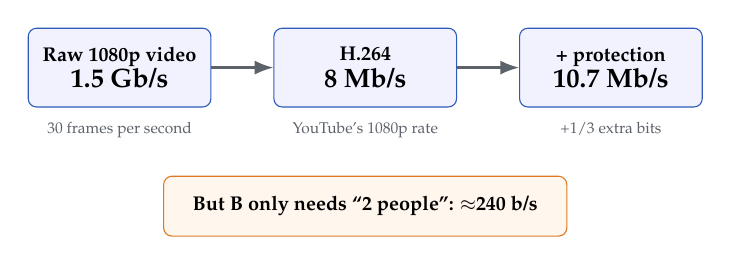
\begin{tikzpicture}[scale=0.8,transform shape,
      box/.style={netnode,minimum width=2.9cm,minimum height=1.25cm,font=\small\bfseries}]
    \node[box] (raw) at (0,0) {Raw 1080p video\\[1pt]{\large 1.5 Gb/s}};
    \node[box,visible on=<2->] (h264) at (3.9,0) {H.264\\[1pt]{\large 8 Mb/s}};
    \node[box,visible on=<3->] (fec) at (7.8,0) {+ protection\\[1pt]{\large 10.7 Mb/s}};
    \draw[flow,visible on=<2->] (raw) -- (h264);
    \draw[flow,visible on=<3->] (h264) -- (fec);
    \node[lbl,below=3pt of raw] {30 frames per second};
    \node[lbl,below=3pt of h264,visible on=<2->] {YouTube's 1080p rate};
    \node[lbl,below=3pt of fec,visible on=<3->] {+1/3 extra bits};
    \node[corenode,minimum width=6.4cm,minimum height=0.95cm,font=\small\bfseries,
      visible on=<4->] (b) at (3.9,-2.2) {But B only needs ``2 people'': $\approx$240 b/s};
  \end{tikzpicture}

  \vspace{0.6em}
  \raggedright
  \uncover<5->{\qa{What does the receiver check at the end?}
     {Only whether every bit is right. One wrong bit, and it is sent again.
      Nobody asks what the video shows.}}

  \vspace{0.2em}
  \source{https://support.google.com/youtube/answer/1722171}{YouTube recommended
    upload encoding settings; IEEE Std 802.11; orange box = teaching example}
\end{frame}

% Teaching note (90 s): two reasons this design won. (1) Divide and conquer:
% Shannon's separation theorem says compressing and protecting can be designed
% separately with no loss -- for one sender and one receiver, and only in the limit of
% very long messages. Exact conditions (Cover & Thomas, Elements of Information
% Theory, 2nd ed., Wiley 2006, Thm. 7.13.1): point-to-point, discrete memoryless
% channel, source satisfying the AEP, error probability -> 0 only as block length ->
% infinity. Lossy form: distortion D is achievable if R(D) < C and impossible if
% R(D) > C. Consequence: H.264 does not care whether it rides on Wi-Fi or 5G -- bits are
% a universal interface. (2) A speed limit: capacity C = B log2(1 + SNR); e.g. 20 MHz
% at 20 dB SNR gives about 133 Mb/s. It is a ceiling on reliable bits per second, not
% a calculator for a real radio's rate.
\begin{frame}{Why this design won}
  \vspace{1.4em}
  \begin{columns}[T,onlytextwidth]
    \column{0.48\textwidth}
      \centering
      {\Large\textbf{\textcolor{ranblue}{Divide and conquer}}\par}
      \vspace{0.8em}
      Compress and protect\\separately: \textbf{nothing lost}\\
      {\small\textcolor{softgray}{(long messages, one link)}}
    \column{0.48\textwidth}
      \centering
      \uncover<2->{%
      {\Large\textbf{\textcolor{coreorange}{A speed limit}}\par}
      \vspace{0.8em}
      Every channel has a\\\textbf{maximum reliable rate}\\
      {\small\textcolor{softgray}{$C = B \log_2(1+\mathrm{SNR})$}}}
  \end{columns}

  \vspace{2.2em}
  \takeawayat{3-}{Bits became a universal interface:\\
    any app over any network.}
  \source{https://doi.org/10.1002/j.1538-7305.1948.tb01338.x}{Shannon (1948);
    Cover \& Thomas, Elements of Information Theory, 2nd ed., Thm.\ 7.13.1}
\end{frame}

% Teaching note (170 s): the pictures carry the slide -- one frame per click.
% Real video calls do not just freeze when the signal weakens: WebRTC-style feedback
% adapts. The receiver keeps reporting when each packet arrived (TWCC feedback; in
% libwebrtc the report interval defaults to 100 ms within 50-250 ms -- from an earlier
% reading of the source, recheck before quoting), and the sender's congestion control
% (GCC) estimates the available bandwidth and lowers the encoder's target bitrate, so
% the picture gets blockier rather than stopping (second frame). But the loop always
% reacts after the fact: when wireless capacity drops suddenly, packets queue up at
% the access point before the sender slows down, so frames arrive late -- a latency
% spike -- and the receiver's playout can briefly freeze (WebRTC's own statistics
% count such freezes as freezeCount). That gap between "the channel changed" and "the
% sender reacted" is exactly what Zhuge (Meng et al., "Achieving Consistent Low
% Latency for Wireless Real-Time Communications with the Shortest Control Loop," ACM
% SIGCOMM 2022, doi:10.1145/3544216.3544225) attacks by shortening the control loop
% at the AP. Background if asked: a link with ONE fixed setting and no feedback shows
% the pure all-or-nothing "cliff" (digital TV freezing; old analog TV just got snowy)
% -- learned-JSCC papers often compare against that, but the fair baseline is a
% system with feedback. Theory behind "long messages, one link": at finite
% blocklength separation pays a penalty that joint coding can avoid (Kostina & Verdu,
% IEEE Trans. Inf. Theory 2013, doi:10.1109/TIT.2013.2238657); for a Gaussian source
% over an AWGN channel with matched bandwidth, uncoded transmission is optimal at
% every SNR at once, which no single digital rate can match (Gastpar, Rimoldi &
% Vetterli, IEEE Trans. Inf. Theory 2003, doi:10.1109/TIT.2003.810631).
\begin{frame}{Where it struggles}
  \vspace{0.8em}
  \centering
  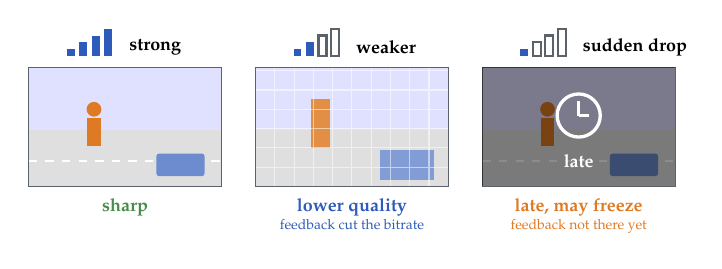
\begin{tikzpicture}[scale=0.72,transform shape]
    \begin{scope}
      \signalbars{0.45}{2.3}{4}
      \node[anchor=west,font=\small\bfseries] at (1.65,2.45) {strong};
      \pic at (0,0) {streetframe};
      \node[font=\small\bfseries,text=softgreen,anchor=north] at (1.7,-0.1) {sharp};
    \end{scope}
    \begin{scope}[visible on=<2->]
      \signalbars{4.45}{2.3}{2}
      \node[anchor=west,font=\small\bfseries] at (5.65,2.45) {weaker};
      \pic at (4,0) {streetblocky};
      \node[font=\small\bfseries,text=ranblue,anchor=north,align=center] at (5.7,-0.1)
        {lower quality\\[-2pt]{\scriptsize\mdseries feedback cut the bitrate}};
    \end{scope}
    \begin{scope}[visible on=<3->]
      \signalbars{8.45}{2.3}{1}
      \node[anchor=west,font=\small\bfseries] at (9.65,2.45) {sudden drop};
      \pic at (8,0) {streetframe};
      \pic at (8,0) {late};
      \node[font=\small\bfseries,text=coreorange,anchor=north,align=center] at (9.7,-0.1)
        {late, may freeze\\[-2pt]{\scriptsize\mdseries feedback not there yet}};
    \end{scope}
  \end{tikzpicture}

  \vspace{0.5em}
  \raggedright
  \begin{itemize}[<+(3)->]\itemsep5pt
    \item \textbf{Feedback adapts --- one step late:} quality drops, delay spikes
    \item \textbf{Every bit counts the same:} sky = pedestrian
    \item \textbf{Receiver B only needs an answer}
  \end{itemize}

  \vspace{0.5em}
  \takeawayat{7-}{Today's video adapts, but after the fact ---\\
    and it always sends everything.}
  \source{https://doi.org/10.1145/3544216.3544225}{Feedback delay on wireless links:
    Z.\ Meng et al., ``Zhuge,'' ACM SIGCOMM 2022}
\end{frame}

%!TEX root = ./main.tex

\section[SemCom]{What Is Semantic Communication?}

% SECTION TIMING: 14:10--22:10 (4 frames): 110 + 140 + 90 + 140 = 480 s.

% Teaching note (110 s): Weaver wrote the companion essay to Shannon's paper and
% split "communication" into three questions. Walk the street-camera example up the
% levels, one click per level: every frame arrives intact (A); the scene is
% understood -- a pedestrian is crossing (B); the car brakes in time (C). Shannon
% answered Level A, on purpose. Then reveal the left tags: today's networks = A,
% version 1 of semantic communication ~ B, version 2 ~ C. Say the caveat once: papers
% use "semantic" loosely for both B and C; the mapping is a teaching aid. Level A
% never disappears -- a semantic system still rides on a physical channel.
% Weaver's exact wording (Sec. 1.2, "Three Levels of Communications Problems"; p. 4
% of the 1963 paperback): A "How accurately can the symbols of communication be
% transmitted?", B "How precisely do the transmitted symbols convey the desired
% meaning?", C "How effectively does the received meaning affect conduct in the
% desired way?" The slide paraphrases them.
\begin{frame}{Weaver 1949: three levels}
  \vspace{0.8em}
  \centering
  {\large A camera streams a street crossing\par}

  \vspace{1.0em}
  % SOURCE: W. Weaver, "Recent Contributions to the Mathematical Theory of
  % Communication," in Shannon & Weaver, The Mathematical Theory of Communication, 1949.
  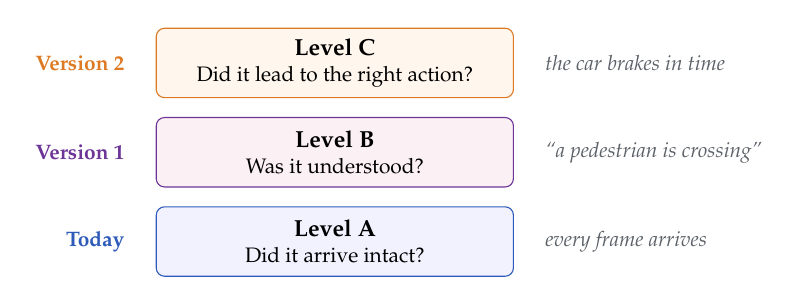
\begin{tikzpicture}[scale=0.84,transform shape,
      lvl/.style={minimum width=5.4cm,minimum height=1.05cm,align=center},
      ex/.style={anchor=west,font=\small\itshape,text=softgray},
      tag/.style={anchor=east,font=\small\bfseries}]
    \node[netnode,lvl] (A) at (0,0) {Level A\\[-1pt]{\small\mdseries Did it arrive intact?}};
    \node[oranode,lvl,visible on=<2->] (B) at (0,1.35)
      {Level B\\[-1pt]{\small\mdseries Was it understood?}};
    \node[corenode,lvl,visible on=<3->] (C) at (0,2.7)
      {Level C\\[-1pt]{\small\mdseries Did it lead to the right action?}};
    \node[ex] at ([xshift=10pt]A.east) {every frame arrives};
    \node[ex,visible on=<2->] at ([xshift=10pt]B.east) {``a pedestrian is crossing''};
    \node[ex,visible on=<3->] at ([xshift=10pt]C.east) {the car brakes in time};
    \node[tag,text=ranblue,visible on=<4->] at ([xshift=-10pt]A.west) {Today};
    \node[tag,text=ranpurple,visible on=<4->] at ([xshift=-10pt]B.west) {Version 1};
    \node[tag,text=coreorange,visible on=<4->] at ([xshift=-10pt]C.west) {Version 2};
  \end{tikzpicture}

  \vspace{1.2em}
  \takeawayat{5-}{Semantic communication aims at Level B or C,\\
    not just Level A.}
  \plainsource{W.\ Weaver, ``Recent Contributions to the Mathematical Theory of
    Communication,'' in Shannon and Weaver, The Mathematical Theory of Communication,
    Univ.\ of Illinois Press, 1949, Sec.\ 1.2 (paraphrased)}
\end{frame}

% Teaching note (140 s): compare with the suitcase slide. The two AI models replace
% compress/protect; what crosses the channel is a compact set of learned "meaning"
% features (real or complex numbers), not a compressed video file. Sender and
% receiver are trained together, with channel noise simulated in the middle, so they
% learn a code that survives it. The green box is the key new requirement: both sides
% must hold the same trained model (papers call it the shared knowledge base:
% weights, training data, context). Analogy: "meet at the usual place" only works
% between friends who share context. In most systems the semantic and channel
% encoders are one neural network trained end to end, called deep joint
% source-channel coding (deep JSCC).
\begin{frame}{A semantic communication system}
  \vspace{1.4em}
  \centering
  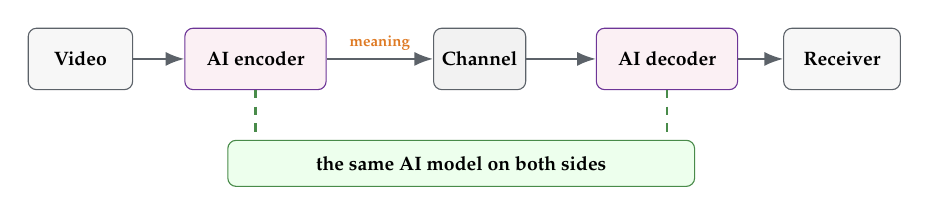
\begin{tikzpicture}[scale=0.78,transform shape]
    \node[endnode] (src) at (0,0) {Video};
    \node[nnnode,minimum width=2.3cm,minimum height=1.0cm,font=\small\bfseries] (enc)
      at (2.85,0) {AI encoder};
    \node[chnode,minimum width=1.5cm,minimum height=1.0cm,font=\small\bfseries] (ch)
      at (6.5,0) {Channel};
    \node[nnnode,minimum width=2.3cm,minimum height=1.0cm,font=\small\bfseries] (dec)
      at (9.55,0) {AI decoder};
    \node[endnode,minimum width=1.9cm] (dst) at (12.4,0) {Receiver};
    \draw[flow] (src) -- (enc);
    \draw[flow] (enc) -- node[above,iface]{meaning} (ch);
    \draw[flow] (ch) -- (dec);
    \draw[flow] (dec) -- (dst);
    \node[kbnode,minimum width=7.6cm,minimum height=0.75cm,font=\small\bfseries,
      visible on=<2->] (kb) at (6.2,-1.7) {the same AI model on both sides};
    \draw[softgreen,thick,dashed,visible on=<2->] (enc.south) -- (enc.south |- kb.north);
    \draw[softgreen,thick,dashed,visible on=<2->] (dec.south) -- (dec.south |- kb.north);
  \end{tikzpicture}

  \vspace{1.6em}
  \uncover<3->{{\large ``Meet at the usual place'' works\\
    only between friends who share context.}\par}

  \vspace{1.6em}
  \takeawayat{4-}{The shared AI model plays the role of shared context.}
  \source{https://doi.org/10.1109/JSAC.2022.3223408}{D.\ G\"und\"uz et al.,
    ``Beyond Transmitting Bits,'' IEEE JSAC, 2023}
\end{frame}

% Teaching note (90 s): make "meaning error" concrete before any neural network
% appears. First answer the obvious objection -- "doesn't the network resend lost
% packets?" (slide "By the numbers" said so). Yes, but a resend costs at least one
% round trip, and live video frames have a playback deadline: data that arrives after
% its frame's deadline is useless for that frame, so it counts as lost. GRACE (NSDI
% 2024) counts packets that miss the decoding deadline as lost, and KDC (NSDI 2026)
% replays the losses that remain after transport-layer retransmission -- loss after
% resending is real in live video. Resending also treats every packet the same: a
% sky packet gets the same retries as a pedestrian packet. Both received frames lost
% exactly the same amount of data -- one small
% block. In the first, the block fell on the sky: nothing anyone cares about is gone.
% In the second, it fell on the pedestrian: a person watching might miss them, and a
% detector might too. Same loss, completely different damage; a traditional receiver
% only counts the lost bits. (Illustration: in real compressed video one lost packet
% can damage a larger area and several following frames, because frames are predicted
% from earlier ones until the next key frame.) Then reveal the fork: two ways to
% define "meaning delivered", which split the rest of the lecture.
\begin{frame}{Same loss, two outcomes}
  \vspace{0.3em}
  \centering
  {\large Each received frame lost the \textbf{same} amount of data.\par}

  \vspace{0.2em}
  {\small\textcolor{softgray}{Live video can't wait for every resend: late data
    counts as lost.}\par}

  \vspace{0.6em}
  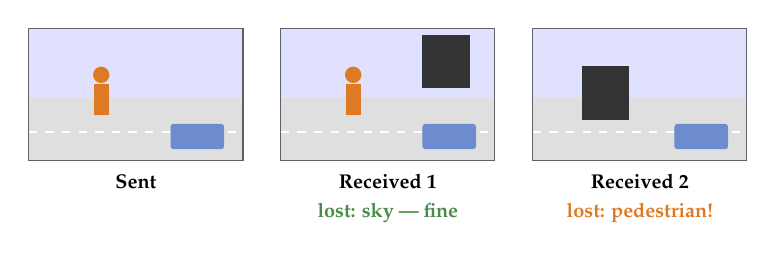
\begin{tikzpicture}[scale=0.8,transform shape]
    \pic at (0,0) {streetframe};
    \node[font=\small\bfseries,anchor=north] at (1.7,-0.1) {Sent};
    \begin{scope}[visible on=<2->]
      \pic at (4.0,0) {streetframe};
      \fill[black!80] (6.25,1.15) rectangle (7.0,2.0);
      \node[font=\small\bfseries,anchor=north] at (5.7,-0.1) {Received 1};
      \node[font=\small\bfseries,text=softgreen,anchor=north] at (5.7,-0.55)
        {lost: sky --- fine};
    \end{scope}
    \begin{scope}[visible on=<3->]
      \pic at (8.0,0) {streetframe};
      \fill[black!80] (8.78,0.65) rectangle (9.53,1.5);
      \node[font=\small\bfseries,anchor=north] at (9.7,-0.1) {Received 2};
      \node[font=\small\bfseries,text=coreorange,anchor=north] at (9.7,-0.55)
        {lost: pedestrian!};
    \end{scope}
  \end{tikzpicture}

  \vspace{0.4em}
  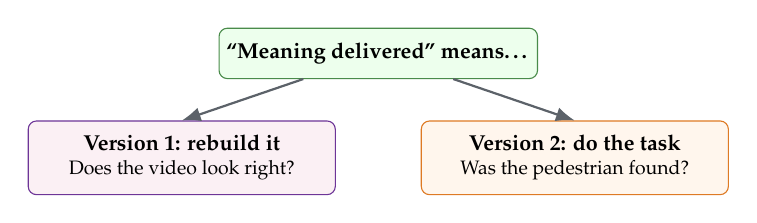
\begin{tikzpicture}[scale=0.78,transform shape,visible on=<4->]
    \node[kbnode,minimum width=3.6cm] (m) at (0,0) {``Meaning delivered'' means\ldots};
    \node[oranode,minimum width=5.0cm,minimum height=1.2cm,align=center] (r)
      at (-3.2,-1.7) {Version 1: rebuild it\\[-1pt]{\small\mdseries Does the video look
      right?}};
    \node[corenode,minimum width=5.0cm,minimum height=1.2cm,align=center] (t)
      at (3.2,-1.7) {Version 2: do the task\\[-1pt]{\small\mdseries Was the pedestrian
      found?}};
    \draw[flow] (m) -- (r.north);
    \draw[flow] (m) -- (t.north);
  \end{tikzpicture}

  \vspace{0.4em}
  \takeawayat{5-}{Same amount of lost data, different damage.}
\end{frame}

% Teaching note (140 s): the "why bother" slide -- two advantages, each with real
% numbers; say "best cases, each against its own baseline" out loud. We will see how
% each system works in the next two parts.
% LESS BANDWIDTH. (1) DVST (Wang et al., IEEE JSAC 2023) rebuilds video and "can save
% up to 50% channel bandwidth cost, compared to classical H.264/H.265 combined with
% LDPC and digital modulation"; it is slightly worse than H.265 + LDPC on some test
% sets. (2) MagicStream (Cheng et al., ACM SenSys 2024, "Bandwidth-conserving
% Immersive Telepresence via Semantic Communication") sends body-pose (SMPL-X) and
% color semantics instead of point clouds: 0.2 Mb/s vs. 72.3 Mb/s for MetaStream's
% point-cloud streaming at its default 200K points per frame (360x); the paper's
% "1195x" applies only when the baseline is pushed to match MagicStream's quality.
% (3) VideoQA-SC (Guo et al., IEEE JSAC 2025) answers questions about video without
% rebuilding it: at low SNR "saving almost 99.5% of the bandwidth" and +5.17% answer
% accuracy vs. a DVST-based system that rebuilds the video first.
% SURVIVES A BAD NETWORK. (4) Signal drops: Deep JSCC (Bourtsoulatze, Kurka &
% Gunduz, IEEE TCCN 2019) "does not suffer from the 'cliff effect'" -- quality
% follows the received signal without any feedback (baseline: JPEG/JPEG2000 + an
% idealized capacity-achieving code, NOT a WebRTC-style adaptive system). (5) Packet loss: GRACE (Cheng et al., USENIX
% NSDI 2024) trains a neural video encoder and decoder together with simulated packet
% loss, so a frame can be decoded from whatever packets arrive; vs. FEC (Tambur on
% H.265) on real LTE traces, with the SAME congestion control for every scheme, it
% "reduces undecodable frames by 95% and stall duration by 90%" (both "up to" figures
% in the evaluation) -- the strongest evidence here against a feedback-based system. GRACE calls itself a neural codec,
% not semantic communication -- it is the same joint-training idea applied to lost
% packets; say so if asked. Survey wording (Gunduz et al., IEEE JSAC 2023): "unlike
% separation-based approaches, their performance does not fall apart when the channel
% quality falls below a certain threshold" -- the same survey calls the field "still
% in its infancy".
\begin{frame}{What we gain}
  \vspace{0.8em}
  \begin{columns}[T,onlytextwidth]
    \column{0.49\textwidth}
      {\Large\textbf{\textcolor{softgreen}{Less bandwidth}}\par}
      \vspace{0.6em}
      \begin{itemize}[<+->]\itemsep7pt
        \item Rebuilt video:\\ \textbf{up to 50\% less}
          {\scriptsize\textcolor{softgray}{(DVST)}}
        \item 3D video call:\\ \textbf{0.2 vs.\ 72 Mb/s}
          {\scriptsize\textcolor{softgray}{(MagicStream)}}
        \item Task only, no video:\\ \textbf{$\approx$99.5\% less}
          {\scriptsize\textcolor{softgray}{(VideoQA-SC)}}
      \end{itemize}
    \column{0.49\textwidth}
      \uncover<4->{{\Large\textbf{\textcolor{coreorange}{Survives a bad network}}\par}}
      \vspace{0.6em}
      \begin{itemize}[<+->]\itemsep7pt
        \item Signal drops:\\ \textbf{blurrier at once, no wait}
          {\scriptsize\textcolor{softgray}{(Deep JSCC)}}
        \item Packet loss, same feedback:\\ \textbf{up to 95\% fewer}\\
          \textbf{broken frames} than FEC {\scriptsize\textcolor{softgray}{(GRACE)}}
      \end{itemize}
  \end{columns}

  \vspace{1.0em}
  \centering
  \uncover<6->{{\small\textcolor{softgray}{Best cases reported by each paper, each
    against its own baseline.}}\par}

  \vspace{0.4em}
  \takeawayat{6-}{Send less, and break less\\ when the network misbehaves.}
  \plainsource{Wang et al., JSAC 2023; Cheng et al., SenSys 2024; Guo et al., JSAC
    2025; Bourtsoulatze et al., TCCN 2019; Cheng et al., NSDI 2024}
\end{frame}

%!TEX root = ./main.tex

\section[Rebuild]{Version 1: Reconstruction-Oriented}

% SECTION TIMING: 22:10--30:30 (4 frames): 170 + 130 + 110 + 90 = 500 s.
% Flex: "Weak signal" can drop to 90 s (skip the third bullet's explanation).

% Teaching note (170 s): a CONCEPT slide, not a paper slide -- "how does Version 1
% actually work?" Mention the research name once (deep joint source-channel coding,
% "deep JSCC") so students recognize it in papers, then teach the idea.
% Background: the founding example of learned reconstruction (Deep JSCC =
% deep joint source-channel coding). Trace one image left to right: an encoder
% network maps the pixel values straight to radio symbols (complex numbers); the
% channel adds noise; a decoder network outputs an approximate image. There is no
% JPEG, no error-correcting code, and no checksum. Training: show it many images,
% simulate noise in the middle (a fixed, non-trainable layer), and reward a close copy
% (mean squared error); gradients flow through the noise layer, so both networks learn
% together. Paper details if asked: CNN encoder/decoder; power normalization so the
% average transmit power is P; "bandwidth compression ratio" k/n (channel symbols per
% source value), e.g. k/n = 1/6 on CIFAR-10 (32x32x3 = 3072 values -> 512 symbols);
% evaluated with PSNR and SSIM; also tested on Kodak images. It works on single
% images; a video is a sequence of images, and video versions follow two slides later.
\begin{frame}{How Version 1 works: practice with noise}
  \vspace{1.6em}
  \centering
  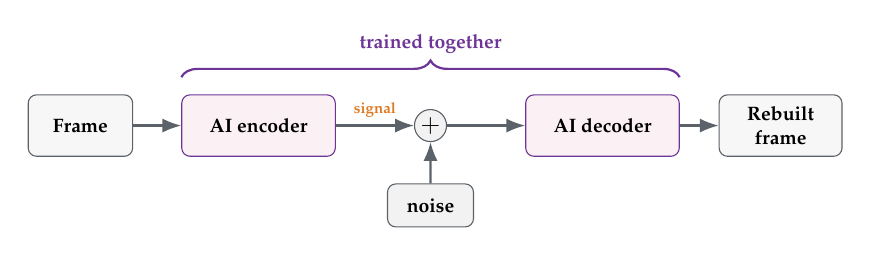
\begin{tikzpicture}[scale=0.78,transform shape]
    \node[endnode] (x) at (0,0) {Frame};
    \node[nnnode,minimum width=2.5cm,minimum height=1.0cm,font=\small\bfseries] (enc)
      at (2.9,0) {AI encoder};
    \node[draw=softgray,fill=gray!10,circle,inner sep=1pt,font=\large\bfseries] (plus)
      at (5.7,0) {$+$};
    \node[chnode,minimum width=1.4cm,minimum height=0.7cm,font=\small\bfseries] (w)
      at (5.7,-1.3) {noise};
    \node[nnnode,minimum width=2.5cm,minimum height=1.0cm,font=\small\bfseries] (dec)
      at (8.5,0) {AI decoder};
    \node[endnode,minimum width=2.0cm] (xh) at (11.4,0) {Rebuilt\\frame};
    \draw[flow] (x) -- (enc);
    \draw[flow] (enc) -- node[above,iface]{signal} (plus);
    \draw[flow] (w) -- (plus);
    \draw[flow] (plus) -- (dec);
    \draw[flow] (dec) -- (xh);
    \draw[decorate,decoration={brace,amplitude=6pt},thick,ranpurple]
      ([yshift=8pt]enc.north west) -- ([yshift=8pt]dec.north east)
      node[midway,above=7pt,font=\small\bfseries,text=ranpurple] {trained together};
  \end{tikzpicture}

  \vspace{1.4em}
  \raggedright
  \begin{itemize}[<+(1)->]\itemsep8pt
    \item One AI replaces ``compress, then protect''
    \item Training: add noise on purpose, reward a close copy
  \end{itemize}

  \vspace{1.4em}
  \takeawayat{4-}{Like two partners practicing a code\\
    until it survives a noisy phone line.}
  \source{https://arxiv.org/abs/1809.01733}{First shown for images (``deep JSCC''):
    Bourtsoulatze, Kurka \& G\"und\"uz, IEEE TCCN, 2019}
\end{frame}

% Teaching note (130 s): the same three situations as "Where it struggles". First
% click: today's row with feedback (WebRTC-style) -- sharp; blockier once feedback has
% cut the bitrate; late (latency spike, maybe a brief freeze) right after a sudden
% drop, before feedback reacts. Second click: the Version 1 row (the 2019 deep JSCC
% result) -- sharp, a bit soft,
% blurrier. The encoder does not change and no feedback is needed: the picture simply
% gets softer as the received signal gets worse, at the moment it happens. The
% pictures are a sketch, not output from the paper. Be honest about the evidence: the
% 2019 paper's claims (abstract) are against digital schemes WITHOUT feedback -- on
% an AWGN channel it beats JPEG/JPEG2000 + an IDEALIZED capacity-achieving code at low
% SNR and low bandwidth, and it degrades gracefully as the test SNR moves away from
% the training SNR (no cliff); on slow Rayleigh fading it is ahead at every SNR and
% bandwidth tested. It was NOT compared with WebRTC-style feedback. The stronger
% evidence against adaptive systems is GRACE (slide "What we gain"): same congestion
% control, fewer undecodable frames and stalls on real LTE traces. With a strong,
% stable signal and enough bandwidth, classic coding can be sharper.
\begin{frame}{Weak signal: no waiting for feedback}
  \vspace{0.6em}
  \centering
  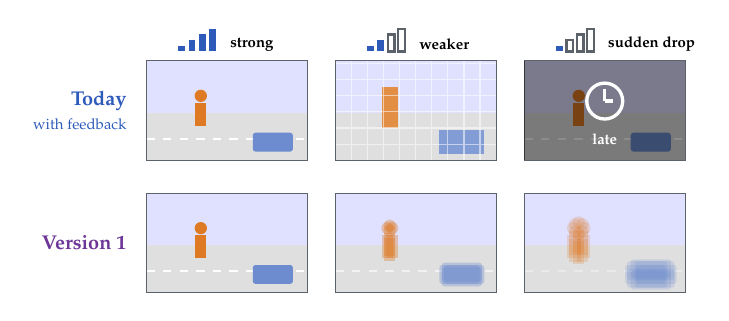
\begin{tikzpicture}[scale=0.6,transform shape]
    \signalbars{0.45}{2.3}{4}
    \node[anchor=west,font=\small\bfseries] at (1.65,2.45) {strong};
    \signalbars{4.45}{2.3}{2}
    \node[anchor=west,font=\small\bfseries] at (5.65,2.45) {weaker};
    \signalbars{8.45}{2.3}{1}
    \node[anchor=west,font=\small\bfseries] at (9.65,2.45) {sudden drop};
    \node[anchor=east,font=\large\bfseries,text=ranblue,align=right] at (-0.3,1.05)
      {Today\\{\small\mdseries with feedback}};
    \pic at (0,0) {streetframe};
    \pic at (4,0) {streetblocky};
    \pic at (8,0) {streetframe};
    \pic at (8,0) {late};
    \begin{scope}[visible on=<2->]
      \node[anchor=east,font=\large\bfseries,text=ranpurple,align=right]
        at (-0.3,-1.75) {Version 1};
      \pic at (0,-2.8) {streetframe};
      \pic at (4,-2.8) {streetsoft};
      \pic at (8,-2.8) {streetblurry};
    \end{scope}
  \end{tikzpicture}

  {\scriptsize\textcolor{softgray}{Sketch, not output from the paper.}\par}

  \vspace{0.5em}
  \raggedright
  \begin{itemize}[<+(2)->]\itemsep5pt
    \item Picture follows the signal \textbf{at once} --- no feedback round trip
    \item Strong, stable signal: classic coding can be sharper
  \end{itemize}

  \vspace{0.5em}
  \takeawayat{5-}{Its strength is reacting instantly,\\
    not ``always better.''}
  \source{https://arxiv.org/abs/1809.01733}{Bourtsoulatze, Kurka, G\"und\"uz,
    IEEE TCCN, 2019 (compared with digital schemes without feedback)}
\end{frame}

% Teaching note (110 s): Version 1 for video -- again a concept slide; DVST is the
% research system that shows it. DVST (Wang et al., "Wireless Deep
% Video Semantic Transmission," IEEE JSAC 41(1), 2023) rebuilds video for viewing.
% Each frame is encoded with the previous frame as context, so mostly what is new gets
% sent; the features go out with deep JSCC, and more channel bandwidth goes to frames
% and regions that are harder to code. Headline (paper's introduction): it "can save
% up to 50% channel bandwidth cost, compared to classical H.264/H.265 combined with
% LDPC and digital modulation schemes"; in the detailed comparison (AWGN, 10 dB) it
% needs 40-80% of the bandwidth of H.264 + LDPC at equal PSNR. Say the caveats the
% paper itself reports: slightly worse than H.265 + LDPC on some test sets (HEVC
% classes C and E), only close to the ideal H.265 + capacity-achieving-code bound, and
% only P-frames are evaluated. Note it still rebuilds every frame -- which is exactly
% what Version 2 will skip.
\begin{frame}{Version 1 for video: send what's new}
  \vspace{1.2em}
  \centering
  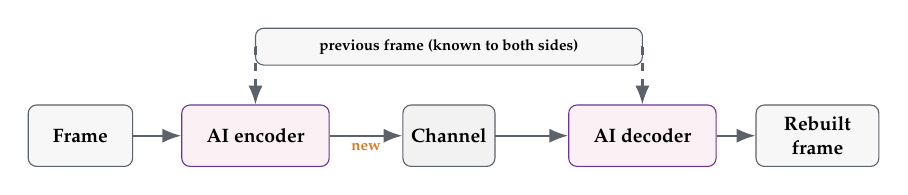
\begin{tikzpicture}[scale=0.78,transform shape]
    \node[endnode] (x) at (0,0) {Frame};
    \node[nnnode,minimum width=2.4cm,minimum height=1.0cm,font=\small\bfseries] (enc)
      at (2.85,0) {AI encoder};
    \node[chnode,minimum width=1.5cm,minimum height=1.0cm,font=\small\bfseries] (ch)
      at (6.0,0) {Channel};
    \node[nnnode,minimum width=2.4cm,minimum height=1.0cm,font=\small\bfseries] (dec)
      at (9.15,0) {AI decoder};
    \node[endnode,minimum width=2.0cm] (xh) at (12.0,0) {Rebuilt\\frame};
    \node[endnode,minimum width=6.3cm,minimum height=0.6cm,font=\scriptsize\bfseries]
      (prev) at (6.0,1.45) {previous frame (known to both sides)};
    \draw[flow] (x) -- (enc);
    \draw[flow] (enc) -- node[below,iface]{new} (ch);
    \draw[flow] (ch) -- (dec);
    \draw[flow] (dec) -- (xh);
    \draw[flow,dashed] (prev.west) -| (enc.north);
    \draw[flow,dashed] (prev.east) -| (dec.north);
  \end{tikzpicture}

  \vspace{1.2em}
  \raggedright
  \begin{itemize}[<+(1)->]\itemsep8pt
    \item Uses the previous frame as context: sends mostly \textbf{what is new}
    \item Gives more bandwidth to frames that are hard to code
    \item \textbf{Up to 50\% less bandwidth} than H.264/H.265 + error coding
  \end{itemize}

  \vspace{0.8em}
  \takeawayat{5-}{Same video, up to half the bandwidth ---\\
    but every frame is still rebuilt.}
  \source{https://doi.org/10.1109/JSAC.2022.3221977}{Example system: DVST, S.\ Wang et
    al., ``Wireless Deep Video Semantic Transmission,'' IEEE JSAC, 2023}
\end{frame}


% Teaching note (90 s): four costs, one click each. (1) Deep JSCC emits arbitrary
% complex values, while Wi-Fi and 5G radios send points from a fixed QAM
% constellation (a fixed "alphabet"); deployable versions must be constrained to that
% alphabet (e.g., DeepJSCC-Q, Tung et al., IEEE JSAIT 2022). (2) Both sides need the
% same trained model, so it must be shipped, versioned, and retrained when content
% shifts (cats -> X-rays). (3) Fair comparison means a modern codec + error
% correction + link adaptation + application feedback (e.g., WebRTC congestion
% control), not one fixed setting. (4) The bit pipe has a
% checksum; there is no checksum for meaning, so a wrong picture arrives without an
% error flag. Generative decoders make point 4 sharper: the sender transmits only a
% compact sketch of the scene (in Grassucci et al. a semantic map saying which object
% class each pixel belongs to) and a diffusion model paints in the details -- the
% result looks real, but some details are the model's guesses (police-sketch-artist
% analogy). "Invented details" is our inference from the perception-distortion
% tradeoff (Blau & Michaeli, CVPR 2018, doi:10.1109/CVPR.2018.00652). Source:
% Grassucci, Barbarossa, Comminiello, "Generative Semantic Communication: Diffusion
% Models Beyond Bit Recovery," IEEE TCCN, 2026, doi:10.1109/TCCN.2026.3689849.
\begin{frame}{The price of rebuilding}
  \vspace{0.8em}
  \begin{enumerate}[<+->]\itemsep8pt
    \item \textbf{Radios only speak a fixed ``alphabet''}\\
      {\small\textcolor{softgray}{learned signals must be squeezed into it}}
    \item \textbf{Both sides need the same AI model}\\
      {\small\textcolor{softgray}{update it on every phone and server}}
    \item \textbf{Fair comparisons are tricky}\\
      {\small\textcolor{softgray}{compare with adaptive systems like WebRTC}}
    \item \textbf{No checksum for meaning}\\
      {\small\textcolor{softgray}{a wrong frame looks fine; generative AI may
        invent details}}
  \end{enumerate}

  \vspace{1.0em}
  \takeawayat{5-}{Smooth quality is paid for with\\
    compatibility, shared models, and trust.}
  \source{https://doi.org/10.1109/JSAIT.2022.3231042}{Point 1: T.-Y.\ Tung et al.,
    ``DeepJSCC-Q: Constellation Constrained Deep JSCC,'' IEEE JSAIT, 2022}
\end{frame}

%!TEX root = ./main.tex

\section[Task]{Version 2: Task-Oriented}

% SECTION TIMING: 30:30--39:40 (4 frames): 130 + 160 + 140 + 120 = 550 s.
% Flex: "Send only when the answer changes" can drop to 45 s (show the ticks, skip AoI).

% Teaching note (130 s): return to Receiver B from the opening slide: it never needs
% to watch the video, it needs to know whether (and where) there are pedestrians.
% Reveal the three options one at a time. Send the video (compressed 1080p video is
% several megabits per second, see the "by the numbers" slide): the server decodes
% every frame and does all the work. Send only the answer (a few bytes per frame):
% the camera must be strong enough to run the whole AI model. Send just enough
% clues: split the model -- first layers on the camera, the rest on the server
% (split computing; Neurosurgeon, Kang et al., ASPLOS 2017, picks the split layer) --
% and train the split together with a simulated noisy channel (BottleNet++, Shao &
% Zhang, IEEE ICC Workshops 2020, puts a fixed channel layer between encoder and
% decoder). That last option is task-oriented semantic communication, and note what
% is missing: no frame is ever rebuilt at the server.
\begin{frame}{Version 2: when the receiver is a machine}
  \vspace{1.0em}
  \centering
  {\large Receiver B only asks: \textbf{``any pedestrians?''}\par}

  \vspace{1.0em}
  \raggedright
  \begin{enumerate}[<+->]\itemsep8pt
    \item \textbf{Send the video} \textcolor{softgray}{(several Mb/s)}:
      the server does all the work
    \item \textbf{Send only the answer} \textcolor{softgray}{(a few bytes)}:
      camera runs the whole AI
    \item \textbf{\textcolor{coreorange}{Send just enough clues}}: split the AI,
      train it with the channel
  \end{enumerate}

  \vspace{0.8em}
  \centering
  
\begin{tikzpicture}[scale=0.76,transform shape,visible on=<3->]
    \node[endnode] (img) at (0,0) {Video};
    \node[nnnode,minimum width=2.4cm,minimum height=1.0cm,font=\small\bfseries] (head)
      at (2.8,0) {AI part 1\\[-2pt]{\scriptsize\mdseries on the camera}};
    \node[chnode,minimum width=1.5cm,minimum height=1.0cm,font=\small\bfseries] (ch)
      at (6.3,0) {Channel};
    \node[nnnode,minimum width=2.4cm,minimum height=1.0cm,font=\small\bfseries] (tail)
      at (9.4,0) {AI part 2\\[-2pt]{\scriptsize\mdseries on the server}};
    \node[corenode,minimum width=2.2cm,minimum height=1.0cm] (out) at (12.4,0)
      {``2 people''};
    \draw[flow] (img) -- (head);
    \draw[flow] (head) -- node[above,iface]{clues} (ch);
    \draw[flow] (ch) -- (tail);
    \draw[flow] (tail) -- (out);
  \end{tikzpicture}

  \vspace{0.8em}
  \takeawayat{4-}{With clues, no frame is ever rebuilt ---\\
    only the decision matters.}
  \source{https://doi.org/10.1145/3037697.3037698}{Kang et al., Neurosurgeon,
    ASPLOS 2017; Shao \& Zhang, BottleNet++, ICC Workshops 2020}
\end{frame}

% Teaching note (160 s): the principled version of "keep only what the task needs",
% called the information bottleneck. Squeeze each frame through a narrow neck so only
% what the task needs survives. The pedestrian example is an illustration of the
% principle: the cited paper (Shao, Mao & Zhang, IEEE JSAC 2022) demonstrated it on
% image classification (MNIST, CIFAR-10), and real learned features are not
% human-readable "shapes of people". The knob (beta in the paper) sets how tight the
% neck is: tighter means fewer symbols on air and, past some point, more mistakes.
% Side effect worth one sentence: less of the video leaves the camera (a privacy
% benefit, not a guarantee). Paper details if asked: objective
% L_IB = -I(Z^;Y) + beta * I(Z^;X), terms labelled "distortion" and "rate", with Z^
% the noisy received feature; variational bounds and a log-uniform sparsity prior
% switch off unneeded feature dimensions; a variable-length variant (VL-VFE) adapts
% how many dimensions are sent to the channel condition. If asked whether one general
% model can serve many tasks: yes, it is an active direction -- e.g., U-DeepSC (Zhang,
% Hu, Qin, Cai, Yu & Tao, "A Unified Multi-Task Semantic Communication System for
% Multimodal Data," IEEE Trans. Commun., 2024, doi:10.1109/TCOMM.2024.3364990) serves
% many tasks with one model, with performance comparable to task-specific systems and
% less overhead and model size than storing one model per task; its abstract states the
% motivating limitation (networks "have to be updated when the task is changed"). The
% trade-off: a general model must keep more information (U-DeepSC adjusts how many
% symbols each task gets), so it sends more bits and needs more compute than a funnel
% built for one task. Large foundation models as the shared knowledge base are another
% direction (e.g., Jiang et al., IEEE Wireless Commun., 2024,
% doi:10.1109/MWC.001.2300346 -- bibliographic check only).
\begin{frame}{How Version 2 works: keep what the task needs}
  \vspace{1.2em}
  \centering
  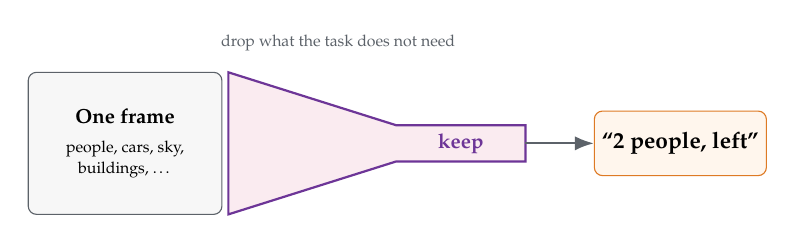
\begin{tikzpicture}[scale=0.82,transform shape]
    \node[endnode,minimum width=3.0cm,minimum height=2.2cm] (x) at (0,0)
      {One frame\\[2pt]{\scriptsize\mdseries people, cars, sky,}\\[-2pt]
       {\scriptsize\mdseries buildings, \ldots}};
    \draw[ranpurple,thick,fill=purple!8] (1.6,1.1) -- (4.2,0.28) -- (6.2,0.28)
      -- (6.2,-0.28) -- (4.2,-0.28) -- (1.6,-1.1) -- cycle;
    \node[font=\small\bfseries,text=ranpurple] at (5.2,0) {keep};
    \node[lbl] at (3.3,1.55) {drop what the task does not need};
    \node[corenode,minimum width=2.4cm,minimum height=1.0cm] (y) at (8.6,0)
      {``2 people, left''};
    \draw[flow] (6.2,0) -- (y.west);
  \end{tikzpicture}

  \vspace{1.2em}
  \raggedright
  \begin{itemize}[<+(1)->]\itemsep8pt
    \item Finding people? Keep their shapes, drop the sky
    \item A knob sets the neck: tighter = fewer bits, more mistakes
  \end{itemize}

  \vspace{1.0em}
  \takeawayat{4-}{Send ``2 people, left'' instead of every pixel.}
  \source{https://arxiv.org/abs/2102.04170}{The ``information bottleneck'' approach:
    J.\ Shao, Y.\ Mao, J.\ Zhang, IEEE JSAC, 2022}
\end{frame}

% Teaching note (140 s): the concrete example of "no frame is ever rebuilt".
% Shao, Zhang & Zhang, "Task-Oriented Communication for Edge Video Analytics," IEEE
% Trans. Wireless Commun. 23(5), 2024 (arXiv 2211.14049): several cameras watch the
% same square (Wildtrack dataset, 7 cameras) and the server predicts where the
% pedestrians are (occupancy map). Devices "transmit the informative features to an
% edge server for processing, rather than reconstructing the videos at the edge
% server". Mechanisms: an information bottleneck keeps only task-relevant features and
% penalizes their bit cost; each frame's features are coded using the previous
% frames' features as side information (send what is new); the server fuses current
% and previous frames. Number on the slide: at the same accuracy (MODA about 85%),
% a learned image codec needs about 130 KB while their method needs 50 KB or 20 KB,
% i.e., 2.6x-6.5x less (our arithmetic). The paper also compares JPEG, WebP, H.264
% (AVC) and H.265 (HEVC) baselines, but only in figures, so no number is quoted here.
% Second example: VideoQA-SC (Guo et al., IEEE JSAC 43(7), 2025): answers questions
% about video clips while "bypassing the need for video reconstruction"; at low SNR
% it improves answer accuracy by 5.17% "while saving almost 99.5% of the bandwidth",
% compared with a DVST-based system that rebuilds the video first.
% Networking cousins (if students ask): DDS (SIGCOMM 2020, up to 59% less bandwidth),
% Reducto (SIGCOMM 2020, drops 51-97% of frames on the camera) and AccMPEG (MLSys
% 2022) send less video for analytics, but the server still decodes ordinary H.264
% video -- a step toward task-oriented communication without leaving the bit pipe.
\begin{frame}{Version 2 for video: no frames rebuilt}
  \vspace{1.0em}
  \centering
  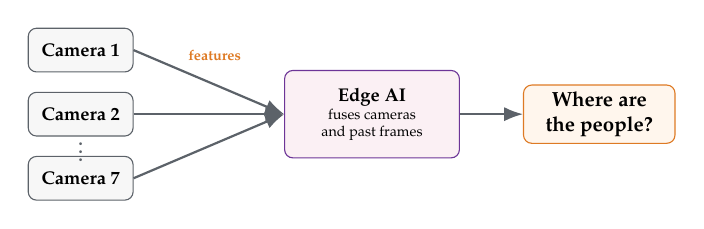
\begin{tikzpicture}[scale=0.74,transform shape]
    \node[endnode,minimum width=1.8cm,minimum height=0.75cm] (c1) at (0,1.1) {Camera 1};
    \node[endnode,minimum width=1.8cm,minimum height=0.75cm] (c2) at (0,0) {Camera 2};
    \node[endnode,minimum width=1.8cm,minimum height=0.75cm] (c7) at (0,-1.1) {Camera 7};
    \node[font=\large,text=softgray] at (0,-0.55) {$\vdots$};
    \node[nnnode,minimum width=3.0cm,minimum height=1.5cm,font=\small\bfseries] (srv)
      at (5.0,0) {Edge AI\\[-2pt]{\scriptsize\mdseries fuses cameras}\\[-3pt]{\scriptsize\mdseries and past frames}};
    \node[corenode,minimum width=2.6cm,minimum height=1.0cm] (out) at (8.9,0)
      {Where are\\the people?};
    \draw[flow] (c1.east) -- (srv.west);
    \draw[flow] (c2.east) -- (srv.west);
    \draw[flow] (c7.east) -- (srv.west);
    \node[iface] at (2.3,1.0) {features};
    \draw[flow] (srv) -- (out);
  \end{tikzpicture}

  \vspace{0.8em}
  \raggedright
  \begin{itemize}[<+(1)->]\itemsep5pt
    \item Cameras send \textbf{features, not video}: no frame is rebuilt
    \item Each feature coded with the previous one: send what is new
    \item Same accuracy, \textbf{2.6--6.5$\times$ less data} than sending
      compressed frames
    \item Video Q\&A: \textbf{$\approx$99.5\% less bandwidth} than rebuilding first
  \end{itemize}

  \vspace{0.5em}
  \takeawayat{6-}{For machines, skip the pixels.}
  \source{https://doi.org/10.1109/TWC.2023.3314888}{Shao, Zhang \& Zhang, IEEE TWC,
    2024; Guo et al., ``VideoQA-SC,'' IEEE JSAC, 2025}
\end{frame}


% Teaching note (120 s): an EXTRA lever, not the definition. Task-oriented
% communication is first about WHAT to send (task-relevant clues, previous slides);
% most task-oriented systems -- including the video-analytics example on the previous slide
% -- still send something for every frame, just far fewer bits. Deciding WHEN to send
% comes from a related research line on timely, goal-oriented status updates. Click
% through: the number of pedestrians in view changes twice; reporting every second
% sends ten updates; reporting only when the answer changes sends three. Three
% catches to say out loud: (1) to know that the answer changed, the camera must
% compute the answer itself (option 2 on "Version 2: when the receiver is a machine") or use a
% cheap change check -- e.g., Reducto (ACM SIGCOMM 2020) drops 51-97% of frames on the
% camera with cheap frame differencing, though it still sends ordinary H.264 frames;
% (2) silence is ambiguous -- "nothing changed" or "the camera died?" -- so real
% systems also send occasional heartbeat messages; (3) if one update is lost, the
% server stays wrong until the next change -- the Age of Incorrect Information metric
% (Maatouk, Kriouile, Assaad & Ephremides, IEEE/ACM Trans. Networking 28(5), 2020,
% doi:10.1109/TNET.2020.3005549) measures exactly that. Age of Information (AoI)
% measures freshness: Delta(t) = t - u(t), where u(t) is when the newest delivered
% update was generated (Yates et al. survey, IEEE JSAC 2021); AoI was introduced by
% Kaul, Gruteser, Rai, Kenney (IEEE SECON 2011) and first analyzed with queueing
% theory by Kaul, Yates, Gruteser (IEEE INFOCOM 2012). The semantic step beyond it
% (Kountouris & Pappas, IEEE Commun. Mag. 2021): freshness alone ignores how the
% source changes; judge an update by its usefulness for the receiver's goal.
\begin{frame}{Send only when the answer changes}
  \vspace{0.6em}
  \centering
  {\small\textcolor{softgray}{An extra option, not a rule: many task-oriented systems
    still send something every frame.}\par}

  \vspace{0.6em}
  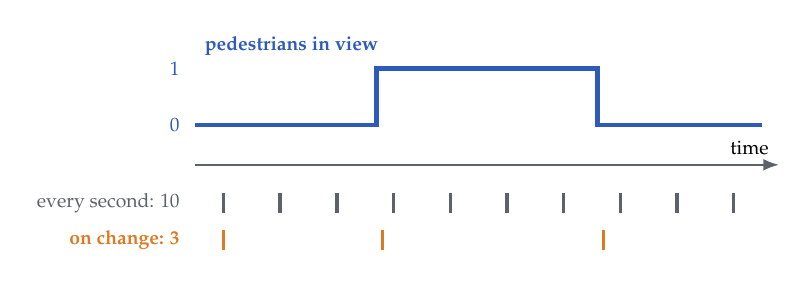
\begin{tikzpicture}[scale=0.72]
    \draw[-{Latex[length=2mm]},thick,softgray] (0,0) -- (10.3,0)
      node[anchor=south east,font=\scriptsize,text=black]{time};
    \draw[ranblue,ultra thick] (0,0.7) -- (3.2,0.7) -- (3.2,1.7) -- (7.1,1.7)
      -- (7.1,0.7) -- (10,0.7);
    \node[font=\scriptsize\bfseries,text=ranblue,anchor=south west] at (0,1.75)
      {pedestrians in view};
    \node[font=\scriptsize,text=ranblue,anchor=east] at (-0.1,0.7) {0};
    \node[font=\scriptsize,text=ranblue,anchor=east] at (-0.1,1.7) {1};
    \foreach \t in {0.5,1.5,...,9.5}{
      \draw[softgray,very thick,visible on=<2->] (\t,-0.5) -- (\t,-0.85);
    }
    \node[font=\scriptsize,text=softgray,anchor=east,visible on=<2->] at (-0.1,-0.67)
      {every second: 10};
    \foreach \t in {0.5,3.3,7.2}{
      \draw[coreorange,very thick,visible on=<3->] (\t,-1.15) -- (\t,-1.5);
    }
    \node[font=\scriptsize\bfseries,text=coreorange,anchor=east,visible on=<3->]
      at (-0.1,-1.32) {on change: 3};
  \end{tikzpicture}

  \vspace{1.0em}
  \raggedright
  \begin{itemize}[<+(3)->]\itemsep6pt
    \item \textbf{Freshness:} how old is my latest update?
      \textcolor{softgray}{(``Age of Information'')}
    \item \textbf{Usefulness:} does this update change what I do?
  \end{itemize}

  \vspace{0.8em}
  \takeawayat{6-}{Another lever: decide \textbf{when} to send, too.}
  \source{https://doi.org/10.1109/JSAC.2021.3065072}{Yates et al., AoI survey,
    IEEE JSAC, 2021; Kountouris \& Pappas, IEEE Commun.\ Mag., 2021}
\end{frame}

%!TEX root = ./main.tex

\section[Hybrid]{Version 3: Meaning-Aware Bits}

% SECTION TIMING: 39:40--43:10 (2 frames): 100 + 110 = 210 s.

% Teaching note (100 s): Version 3 keeps today's pipeline -- standard codec, standard
% network -- and changes only WHERE the bits go. An AI on the camera marks what
% matters for the task; the standard encoder (JPEG/H.264) spends more bits there and
% fewer on the rest; an AI at the receiver fills in what was dropped or lost. It does
% not climb Weaver's levels: it keeps Level A's pipe and uses Level B/C knowledge to
% decide which bits matter most. Tie back to "Same loss, two outcomes" (the
% pedestrian deserves more protection than the sky) and to "Where it struggles"
% ("every bit counts the same"). Why it matters for an edge-networks course: it needs
% nothing new in radios, codecs, or protocols, so it is the easiest kind to deploy.
% Networking cousins (verified earlier): AccMPEG (MLSys 2022) gives higher quality to
% the macroblocks that matter for accuracy; DDS (ACM SIGCOMM 2020) sends a
% low-quality stream and re-sends important regions in high quality; MPEG's Video
% Coding for Machines (ISO/IEC 23888-2) codes video for machine analysis.
\begin{frame}{Version 3: keep the pipe, spend bits by meaning}
  \vspace{1.0em}
  \centering
  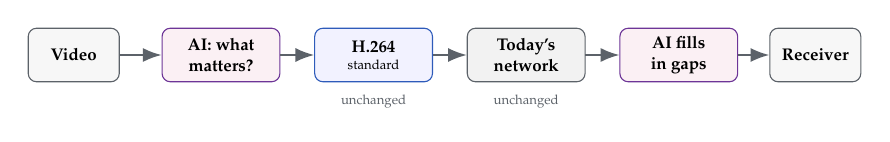
\begin{tikzpicture}[scale=0.68,transform shape,
      std/.style={netnode,minimum width=2.2cm,minimum height=1.0cm,font=\small\bfseries},
      ai/.style={nnnode,minimum width=2.2cm,minimum height=1.0cm,font=\small\bfseries}]
    \node[endnode] (v) at (0,0) {Video};
    \node[ai] (score) at (2.75,0) {AI: what\\matters?};
    \node[std] (enc) at (5.6,0) {H.264\\[-2pt]{\scriptsize\mdseries standard}};
    \node[chnode,minimum width=2.2cm,minimum height=1.0cm,font=\small\bfseries] (net)
      at (8.45,0) {Today's\\network};
    \node[ai] (fill) at (11.3,0) {AI fills\\in gaps};
    \node[endnode] (rx) at (13.85,0) {Receiver};
    \draw[flow] (v) -- (score); \draw[flow] (score) -- (enc); \draw[flow] (enc) -- (net);
    \draw[flow] (net) -- (fill); \draw[flow] (fill) -- (rx);
    \node[lbl,below=3pt of enc] {unchanged};
    \node[lbl,below=3pt of net] {unchanged};
  \end{tikzpicture}

  \vspace{0.9em}
  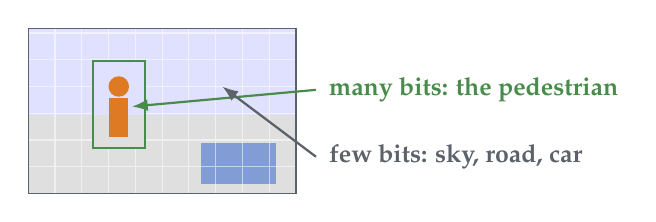
\begin{tikzpicture}[scale=0.85,visible on=<2->]
    \pic at (0,0) {streetv3};
    \draw[-{Latex[length=2mm]},softgreen,thick] (4.3,1.55) -- (1.55,1.3);
    \node[anchor=west,font=\small\bfseries,text=softgreen] at (4.35,1.55)
      {many bits: the pedestrian};
    \draw[-{Latex[length=2mm]},softgray,thick] (4.3,0.55) -- (2.9,1.6);
    \node[anchor=west,font=\small\bfseries,text=softgray] at (4.35,0.55)
      {few bits: sky, road, car};
  \end{tikzpicture}

  \vspace{0.7em}
  \uncover<3->{{\large Nothing new for radios, codecs, or networks.}\par}

  \vspace{0.7em}
  \takeawayat{4-}{Same pipe, smarter spending ---\\
    the easiest version to deploy today.}
\end{frame}

% Teaching note (110 s): one real system, so students see Version 3 works. KDC
% (X. Chen, Z. Feng, W. Zhao, J. Ding, K. Sun, X. Zhang, "From Bits to Tokens:
% Knowledge-Driven Generative Communication of Multimodal Data," USENIX NSDI 2026;
% read in full): a foundation model (CLIP, plus a small language model run once
% offline) turns the task description into keywords -- "autonomous driving" -> car,
% pedestrian, traffic light -- and scores every image patch against them; the
% standard JPEG/H.264 encoder then keeps finer detail in high-scoring regions and
% quantizes the rest coarsely (Sec. 3.2: "fully compatible with H.264/JPEG/PCC and
% existing hardware accelerators"; it runs at the application layer, PHY/MAC and
% retransmissions unchanged); the keywords travel once in a small header; a
% receiver-side restoration network (UNet conditioned on a knowledge base) fills in
% lost or coarse parts. Numbers (Sec. 5.1, images: ImageNet-1K and Cityscapes, 5G
% traces): ~0.85 Top-1 with only 10 kB, close to ~0.87 for the full image, where a
% full JPEG averages ~30 kB; 0.55-0.65 Top-1 at every packet-loss level, while
% progressive JPEG and the learned codec LimitNet fall to <=0.2 at 5-10% loss and the
% semantic system StarFish to ~0.3 at 10% loss (plain JPEG fails). Video (Sec. 5.2,
% driving-video segmentation over real 5G traces): KDC on top of H.264 keeps the
% segmentation score (IoU) 0.1-0.2 higher than plain H.264 under medium-to-high loss.
% Weak spots: it still sends a picture (more bits than Version 2), and it needs AI
% on both ends (the paper reports 32 frames/s on a Jetson Orin).
\begin{frame}{Version 3 in practice}
  \vspace{0.9em}
  \centering
  {\large Example: \textbf{KDC} (NSDI 2026)\par}

  \vspace{0.8em}
  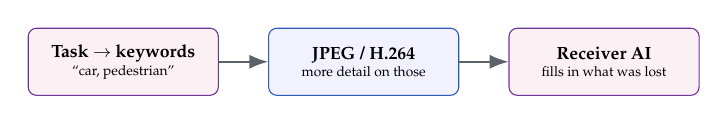
\begin{tikzpicture}[scale=0.71,transform shape,
      st/.style={nnnode,minimum width=3.4cm,minimum height=1.2cm,font=\small\bfseries}]
    \node[st] (a) at (0,0) {Task $\to$ keywords\\[-2pt]{\scriptsize\mdseries ``car, pedestrian''}};
    \node[st,draw=ranblue,fill=blue!5] (b) at (4.3,0)
      {JPEG / H.264\\[-2pt]{\scriptsize\mdseries more detail on those}};
    \node[st] (c) at (8.6,0) {Receiver AI\\[-2pt]{\scriptsize\mdseries fills in what was lost}};
    \draw[flow] (a) -- (b); \draw[flow] (b) -- (c);
  \end{tikzpicture}

  \vspace{0.9em}
  \raggedright
  \begin{itemize}[<+(1)->]\itemsep5pt
    \item Images: near-full accuracy with \textbf{10 kB} \textcolor{softgray}{(a full
      JPEG $\approx$30 kB)}
    \item 10\% packet loss: \textbf{0.55--0.65} accuracy vs.\ \textbf{$\le$0.3} for others
    \item Driving video: H.264 \textbf{+ KDC} beats plain H.264 under loss
  \end{itemize}

  \vspace{0.6em}
  \takeawayat{5-}{Works with today's codecs and networks ---\\
    but still sends a picture, and needs AI on both ends.}
  \source{https://www.usenix.org/conference/nsdi26/presentation/chen-xingyu}{X.\ Chen
    et al., ``From Bits to Tokens: Knowledge-Driven Generative Communication,''
    USENIX NSDI, 2026}
\end{frame}

%!TEX root = ./main.tex

\section[Wrap-up]{Wrap-Up}

% SECTION TIMING: 43:10--50:00 (3 frames): 150 + 160 + 100 = 410 s.
% If behind, show only the first two points of the open-problems frame (90 s).

% Teaching note (150 s): retrieval, not new material -- before each click, ask the
% class to fill in the next row. Rows: today's pipeline reacts one step late and
% sends everything ("Where it struggles"); Version 1 needs the same model on both
% ends and a wrong frame looks fine ("The price of rebuilding"); Version 2 is built
% for the tasks it was trained for -- a new kind of task may need retraining, and
% general multi-task models exist (e.g., U-DeepSC, IEEE Trans. Commun. 2024) but send
% more bits and need more compute -- and there is no video to replay; Version 3 works
% with today's codecs and networks but still sends a picture and needs AI on both
% ends ("Version 3 in practice"). The takeaway answers "which one wins?": none --
% choose by what the receiver needs.
\begin{frame}{Four ways to send video}
  \vspace{0.8em}
  \centering
  {\footnotesize\renewcommand{\arraystretch}{1.45}\setlength{\tabcolsep}{3pt}%
  \begin{tabular}{@{}>{\bfseries}l l l l l@{}}
    \toprule
    & \textbf{Sends} & \textbf{Receiver gets} & \textbf{Strength} & \textbf{Weak spot} \\
    \midrule
    \textcolor{ranblue}{Today}
      & every bit & the exact video & works for any app
      & \makecell[lt]{reacts late;\\sends everything} \\
    \uncover<2->{\textcolor{ranpurple}{Version 1}}
      & \uncover<2->{meaning} & \uncover<2->{a close copy}
      & \uncover<2->{degrades smoothly}
      & \uncover<2->{\makecell[lt]{needs same model;\\errors look fine}} \\
    \uncover<3->{\textcolor{coreorange}{Version 2}}
      & \uncover<3->{task clues} & \uncover<3->{the answer}
      & \uncover<3->{far fewer bits}
      & \uncover<3->{\makecell[lt]{built for its tasks;\\no video to replay}} \\
    \uncover<4->{\textcolor{softgreen}{Version 3}}
      & \uncover<4->{\makecell[lt]{bits, spent\\by meaning}}
      & \uncover<4->{\makecell[lt]{sharp where\\it matters}}
      & \uncover<4->{\makecell[lt]{works on today's\\networks}}
      & \uncover<4->{\makecell[lt]{still sends a picture;\\AI on both ends}} \\
    \bottomrule
  \end{tabular}\par}

  \vspace{1.2em}
  \takeawayat{5-}{No single winner:\\
    choose by what the receiver needs.}
\end{frame}

% Teaching note (160 s): status check, one click per point. Semantic communication
% is research-stage. (1) Today's radios and protocols assume bits (fixed signal
% alphabets, retransmissions, layered stacks). (2) Who trains, ships, and updates the
% shared model on every device? (3) Trust: no checksum for meaning; crafted inputs can
% fool the AI models; transmitted features can still leak private content.
% (4) Standards, checked to about June 2026: 3GPP's AI/ML air-interface work (Rel-18
% study TR 38.843; Rel-19 normative one-sided models) targets CSI feedback/prediction,
% beam management, and positioning; two-sided CSI compression is deferred to Rel-20;
% there is no 3GPP study or work item on semantic communication, and the 6G use-case
% report TR 22.870 mentions it only as motivation inside use cases. 3GPP's other AI
% work (core-network analytics such as NWDAF, AI/ML for NG-RAN) is not about content
% transmission either. Recheck before each delivery of this lecture.
% Version 3 sidesteps the first and last points by design (standard codecs, standard
% networks), which is why it is the closest to deployment today.
% MPEG (the video-codec standards body) is closer to Version 2: Video Coding for
% Machines, VCM (ISO/IEC 23888-2), codes video meant for machine analysis -- its
% decoder still outputs video -- and reached Draft International Standard at MPEG 153
% (January 2026), with the final stage planned for late 2026; Feature Coding for
% Machines, FCM (ISO/IEC 23888-4), codes the intermediate features of a split neural
% network so the cloud "only needs to run the head", and reached Committee Draft at
% MPEG 154 (April-May 2026). These are source-coding standards (no joint design with
% the radio channel). Sources: MPEG press releases for meetings 153-155; stage data
% from the ISS mirror of the ISO record (iso.org itself could not be fetched).
% Optional systems examples if students ask "who builds this?": MagicStream (ACM
% SenSys 2024, semantic 3D telepresence), KDC (USENIX NSDI 2026, knowledge-driven
% generative communication), LITE (ACM SIGCOMM 2026, loss-resilient telepresence with
% multi-modal semantics).
\begin{frame}{Why it is not in your phone yet}
  \vspace{1.2em}
  \begin{enumerate}[<+->]\itemsep12pt
    \item \textbf{Must fit today's radios and networks}
    \item \textbf{Both sides must keep the same AI model}
    \item \textbf{Trust:} no checksum for meaning; AI can be fooled
    \item \textbf{Standards are just starting}\\
      {\small\textcolor{softgray}{no cellular standard yet; MPEG is defining video and
        feature coding \textit{for machines} (2026)}}
  \end{enumerate}

  \vspace{1.6em}
  \takeawayat{5-}{Promising for weak signals and clear goals;\\
    not a replacement for today's networks yet.}
  \source{https://portal.3gpp.org/desktopmodules/Specifications/SpecificationDetails.aspx?specificationId=3983}{3GPP
    TR 38.843 (Rel-18); MPEG press releases, meetings 153--155 (2026)}
\end{frame}

% Teaching note (100 s): four sentences to remember, one click each, then close by
% re-asking the opening question: A needs (a good copy of) the video, B needs only
% the answer. (The pair discussion was removed to make room for Version 3.)
\begin{frame}{Takeaways}
  \vspace{1.2em}
  \begin{enumerate}[<+->]\itemsep10pt
    \item \textbf{\textcolor{ranblue}{Today:}} copy every bit of every frame
    \item \textbf{\textcolor{ranpurple}{Version 1:}} rebuild the video;
      degrades smoothly
    \item \textbf{\textcolor{coreorange}{Version 2:}} no video rebuilt ---
      send only what the task needs
    \item \textbf{\textcolor{softgreen}{Version 3:}} today's pipe,
      bits spent by meaning
  \end{enumerate}

  \vspace{2.0em}
  \askat{5-}{Back to the start: do A and B need the same data?}
\end{frame}


\end{document}
